\documentclass{article}

\usepackage[preprint]{neurips_2025}

\usepackage[utf8]{inputenc}
\usepackage[T1]{fontenc}
\usepackage{hyperref}
\usepackage{url}
\usepackage{booktabs}
\usepackage{amsmath,amssymb,amsfonts}
\usepackage{nicefrac}
\usepackage{microtype}
\usepackage{xcolor}
\usepackage{graphicx}
\usepackage{algorithm}
\usepackage[noend]{algpseudocode}
\usepackage[capitalize,noabbrev]{cleveref}

\makeatletter
\renewcommand{\@noticestring}{Group 10, Department of Computing, The Hong Kong Polytechnic University. COMP6704 Group Project, Fall 2026.}
\makeatother

\newcommand{\R}{\mathbb{R}}
\newcommand{\prox}{\operatorname{prox}}
\newcommand{\argmin}{\operatorname*{argmin}}
\newcommand{\gradnorm}{\|\nabla F(w)\|_2}

\title{Four Solvers, One Objective: A Controlled Comparison of GD, Nesterov, FISTA and ADMM for L2-Regularized Logistic Regression}

\author{%
  LIU Xuyang\\ 26123832r \And
  WANG Zeqing\\ 26029011r \And
  WU Aoqi\\ 26027031r \And
  ZHAO Jixin\\ 26009105r
}

\begin{document}

\maketitle

\begin{abstract}
We train one model, L2-regularized logistic regression, with four convex solvers: gradient descent (GD), Nesterov's accelerated gradient, FISTA and ADMM. All four start from zero, use the same data, and stop at the same full-gradient tolerance $10^{-6}$, which by strong convexity bounds the objective gap by $5\times10^{-11}$. On a synthetic dataset GD is the fastest (12.3\,ms median over 20 runs); on the Wisconsin breast cancer dataset Nesterov and FISTA are the fastest (48.8 and 49.5\,ms) and GD needs more than twice as many updates. We show algebraically that FISTA with an L2 proximal step is the same iteration as Nesterov's method, and the measured trajectories agree. We trace GD's slowness on breast cancer to the global step bound $1/L$, which is about 16 times smaller than the inverse of the largest Hessian eigenvalue at the solution. ADMM with $\rho=1$ needs the fewest outer iterations on breast cancer but is the slowest in time, because each outer iteration contains dense Newton steps. Its runtime changes by more than two orders of magnitude over $\rho\in[0.01,10]$, and at $\rho=\lambda$ it reduces to Newton's method plus residual checks. A fixed budget of 400 updates already gives the final test accuracy on breast cancer while no solver has met the tolerance, so accuracy alone is not a convergence test. Code, raw measurements and figure scripts are available at \url{https://github.com/xuyang-liu16/COMP6704_Group10_Pre}.
\end{abstract}

%======================================================================
\section{Introduction}
\label{sec:intro}

Training a linear classifier is an optimization problem. Given features $x_i$ and labels $y_i$, we choose a weight vector by minimizing an average loss plus a penalty. When the loss and the penalty are convex, every local minimum is global, and with a strongly convex penalty the minimizer is unique \citep{boyd2004convex}. The model that comes out is then fixed by the data and the objective; the solver only decides how much computation it takes to get there. This makes convex model training a clean setting for comparing optimization algorithms: different solvers can be held to the same target and compared on cost alone.

We study L2-regularized logistic regression, one of the most widely used probabilistic classifiers. Its loss is smooth, its gradient costs one pass over the data, and its Hessian has a simple form, so first-order and second-order methods can both be applied and analysed. The project asks a narrow question: \emph{for the same objective, data, starting point and stopping rule, how much work does each of four standard solvers need, and why?}

\paragraph{Background.}
The four solvers come from three lines of work.
\emph{Gradient descent} is the baseline of smooth optimization. With step $1/L$ it has an $O(1/k)$ rate for the objective gap on smooth convex problems and a linear rate $(1-\mu/L)^k$ when the objective is $\mu$-strongly convex \citep{nesterov2004introductory}. Line searches such as Armijo backtracking \citep{armijo1966minimization,nocedal2006numerical} make the step size safe when $L$ is unknown or loose.
\emph{Accelerated gradient methods} add momentum. \citet{nesterov1983method} showed that a look-ahead step improves the worst-case rate to $O(1/k^2)$, which is optimal among first-order methods for smooth convex functions \citep{nesterov2004introductory}. In the strongly convex case a fixed momentum gives a rate depending on $\sqrt{L/\mu}$ instead of $L/\mu$. Without that tuning, momentum methods can oscillate; \citet{odonoghue2015adaptive} proposed adaptive restart as a remedy, and \citet{su2016differential} explained the oscillation through a second-order ODE.
\emph{Proximal and splitting methods} handle objectives of the form $f+g$ in which $g$ may be nonsmooth. The proximal gradient method takes a gradient step on $f$ and then applies the proximal map of $g$ \citep{parikh2014proximal}. FISTA \citep{beck2009fista} adds Nesterov momentum to this step and is the standard solver for L1-regularized problems such as the lasso. ADMM \citep{gabay1976dual,glowinski1975approximation} goes one step further and gives $f$ and $g$ separate copies of the variable, coupled by a linear constraint; \citet{boyd2011admm} survey its use for distributed statistical learning, including logistic regression. Its behaviour depends strongly on the penalty parameter $\rho$, and residual balancing \citep{he2000alternating,boyd2011admm} is a common rule for adapting it.

For large datasets, stochastic gradients are the default tool, and the trade-off between optimization accuracy and statistical accuracy matters \citep{bottou2010large,bottou2018optimization}. We deliberately use full-batch solvers on small datasets. This removes sampling noise, so differences between solvers come from their update rules and per-update cost.

\paragraph{Contributions.}
\begin{itemize}
  \item Four independently written solvers that minimize exactly the same objective, start from the same point and stop on the same full-gradient test. The gradient test gives a certificate on the objective gap for every method (\cref{sec:formulation}).
  \item A short derivation that FISTA with an L2 proximal step and step size $1/L_f$ produces the same iterates as Nesterov's method with step $1/L$, confirmed by overlapping trajectories (\cref{sec:equivalence}).
  \item A timed comparison with 20 repeats, two datasets, five data seeds, an ADMM penalty sweep and a direct Newton control (\cref{sec:results}).
  \item A curvature measurement that explains why GD is slow on breast cancer but competitive on synthetic data, and an explanation of the ADMM case $\rho=\lambda$ (\cref{sec:why-gd,sec:rho}).
\end{itemize}

%======================================================================
\section{Problem formulation}
\label{sec:formulation}

\paragraph{Variables and data.}
Each example $i\in\{1,\dots,n\}$ has standardized features $a_i\in\R^{d-1}$ and a label $y_i\in\{-1,+1\}$. We append a constant $1$, so $x_i=(a_i^\top,1)^\top\in\R^d$, and stack the rows $x_i^\top$ into $X\in\R^{n\times d}$. The variable is $w\in\R^d$, which contains the feature weights and the bias. There are no constraints. The model predicts $P(y_i=+1\mid x_i)=\sigma(x_i^\top w)$ with $\sigma(t)=1/(1+e^{-t})$, and assigns class $+1$ when $x_i^\top w\ge 0$.

\paragraph{Objective.}
For a fixed $\lambda>0$ we solve
\begin{equation}
\label{eq:objective}
\min_{w\in\R^d}\; F(w)=f(w)+g(w),\qquad
f(w)=\frac1n\sum_{i=1}^n\log\!\bigl(1+e^{-y_i x_i^\top w}\bigr),\qquad
g(w)=\frac{\lambda}{2}\|w\|_2^2 .
\end{equation}
The first term is the average negative log-likelihood; the second shrinks the weights. We use $\lambda=0.01$ throughout and also penalize the bias. Penalizing the bias is not the usual choice, but it gives every coordinate curvature at least $\lambda$, which we use below. Since the features are standardized and $\lambda$ is small, its effect on the fitted bias is minor.

\paragraph{Gradient and Hessian.}
Let $p_i=\sigma(x_i^\top w)$ and $b_i=(y_i+1)/2\in\{0,1\}$. Then
\begin{equation}
\label{eq:grad}
\nabla F(w)=\frac1n X^\top(p-b)+\lambda w,\qquad
\nabla^2F(w)=\frac1n X^\top D(w)X+\lambda I,\quad D(w)=\operatorname{diag}\bigl(p_i(1-p_i)\bigr).
\end{equation}
The vector $p-b$ is the prediction error, so the gradient is a correlation between errors and features. One gradient costs $O(nd)$ operations.

\paragraph{Strong convexity and smoothness.}
Every diagonal entry of $D(w)$ lies in $(0,1/4]$. Hence, for all $w$,
\begin{equation}
\label{eq:bounds}
\mu I\preceq \nabla^2F(w)\preceq L I,\qquad
\mu=\lambda,\qquad L=L_f+\lambda,\qquad L_f=\frac{\|X\|_2^2}{4n},
\end{equation}
where $\|X\|_2$ is the largest singular value. The lower bound makes $F$ $\lambda$-strongly convex, so a minimizer $w^\star$ exists and is unique; without the penalty, separable data would let $\|w\|$ grow without bound. The upper bound makes $\nabla F$ $L$-Lipschitz, which justifies the step $1/L$. The ratio $L/\mu$ is a global bound on the condition number; we report it together with the local condition number at $w^\star$ in \cref{sec:why-gd}.

\paragraph{A common stopping rule.}
The optimal value $F^\star$ is unknown, so the objective gap cannot be measured directly. Strong convexity gives a computable bound instead:
\begin{equation}
\label{eq:certificate}
0\le F(w)-F^\star\le \frac{\|\nabla F(w)\|_2^2}{2\lambda}.
\end{equation}
All four solvers therefore stop when $\gradnorm\le 10^{-6}$, evaluated on the full training objective at the returned iterate. By \eqref{eq:certificate} this guarantees $F(w)-F^\star\le 5\times10^{-11}$. For ADMM, the same gradient test is added to its usual residual tests, so a run cannot stop on feasibility alone.

%======================================================================
\section{Methods}
\label{sec:methods}

Each member implemented one solver (\cref{tab:roles}). All start at $w_0=0$. We write $k$ for the update index.

\subsection{Gradient descent (WANG Zeqing)}
GD updates $w_{k+1}=w_k-\eta_k\nabla F(w_k)$. The trial step is $\eta=1/L$; it is accepted if the Armijo condition
$F(w_k-\eta\nabla F(w_k))\le F(w_k)-c\,\eta\,\|\nabla F(w_k)\|_2^2$ holds with $c=10^{-4}$, and halved otherwise. Since $F$ is $L$-smooth, the descent lemma gives a decrease of at least $\|\nabla F\|^2/(2L)$ at $\eta=1/L$, so in exact arithmetic the first trial always satisfies the condition, because $c=10^{-4}<1/2$; the line search is a safeguard. With step $1/L$ and strong convexity,
\begin{equation}
F(w_k)-F^\star\le\Bigl(1-\frac{\mu}{L}\Bigr)^k\bigl(F(w_0)-F^\star\bigr).
\end{equation}
Each update costs one gradient and one objective evaluation, both $O(nd)$.

\subsection{Nesterov's accelerated gradient (LIU Xuyang)}
Nesterov's method takes the gradient at a look-ahead point $v_k$ instead of at $w_k$. With $v_0=w_0$ and $t_0=1$,
\begin{equation}
\label{eq:nesterov}
w_{k+1}=v_k-\frac1L\nabla F(v_k),\qquad
t_{k+1}=\frac{1+\sqrt{1+4t_k^2}}{2},\qquad
v_{k+1}=w_{k+1}+\frac{t_k-1}{t_{k+1}}(w_{k+1}-w_k).
\end{equation}
The momentum weight $(t_k-1)/t_{k+1}$ starts at $0$ and tends to $1$. This is the general-convex schedule, with guarantee $F(w_k)-F^\star=O(L\|w_0-w^\star\|^2/k^2)$ \citep{nesterov1983method,beck2009fista}. It does not use $\mu$ and has no restart. The strongly convex variant with constant momentum $\beta=(\sqrt L-\sqrt\mu)/(\sqrt L+\sqrt\mu)$ has a linear rate governed by $\sqrt{\mu/L}$, but we did not implement it, and we do not claim that rate here. The objective need not decrease monotonically. Each update evaluates the gradient at $v_k$ and, for the stopping test, at $w_{k+1}$: two gradients per update.

\subsection{FISTA (WU Aoqi)}
\label{sec:fista}
FISTA treats $f$ and $g$ separately. It takes a gradient step on $f$ alone, with step $\eta=1/L_f$, and then applies the proximal map of $g$,
\begin{equation}
\prox_{\eta g}(a)=\argmin_{u}\Bigl\{\frac{\lambda}{2}\|u\|^2+\frac{1}{2\eta}\|u-a\|^2\Bigr\}=\frac{a}{1+\eta\lambda}.
\end{equation}
The second equality follows by setting the derivative $\lambda u+(u-a)/\eta$ to zero. The L2 proximal step is therefore a uniform shrinkage of every coordinate, costing $O(d)$. \Cref{alg:fista} lists one run. The penalty enters only through the shrinkage, so the gradient in line 3 must not include $\lambda v_k$; adding it would count the penalty twice. With the same momentum as \eqref{eq:nesterov}, the standard guarantee is $F(w_k)-F^\star\le 2L_f\|w_0-w^\star\|^2/(k+1)^2$ \citep{beck2009fista}. For an L1 penalty the proximal map would be soft-thresholding, which sets small weights exactly to zero; that is the setting FISTA was designed for.

\begin{algorithm}[t]
\caption{FISTA for L2-regularized logistic regression (as implemented)}
\label{alg:fista}
\begin{algorithmic}[1]
\Require $X$, $y$, $\lambda$, tolerance $\varepsilon=10^{-6}$, budget $K$
\State $w_0=v_0=0$, $t_0=1$, $\eta=1/L_f$ with $L_f=\|X\|_2^2/(4n)$
\For{$k=0,1,\dots,K-1$}
  \State $a\gets v_k-\eta\nabla f(v_k)$ \Comment{loss gradient only, $O(nd)$}
  \State $w_{k+1}\gets a/(1+\eta\lambda)$ \Comment{L2 proximal step, $O(d)$}
  \State $t_{k+1}\gets\bigl(1+\sqrt{1+4t_k^2}\bigr)/2$;\quad $v_{k+1}\gets w_{k+1}+\frac{t_k-1}{t_{k+1}}(w_{k+1}-w_k)$
  \If{$\|\nabla F(w_{k+1})\|_2\le\varepsilon$} \textbf{return} $w_{k+1}$ \EndIf
\EndFor
\end{algorithmic}
\end{algorithm}

\subsection{FISTA and Nesterov are the same iteration here}
\label{sec:equivalence}
Write the FISTA update with $\eta=1/L_f$ and multiply numerator and denominator by $L_f$:
\begin{equation}
\label{eq:equivalence}
w_{k+1}=\frac{v_k-\nabla f(v_k)/L_f}{1+\lambda/L_f}
=\frac{L_f v_k-\nabla f(v_k)}{L_f+\lambda}
=v_k-\frac{\nabla f(v_k)+\lambda v_k}{L_f+\lambda}
=v_k-\frac{1}{L}\nabla F(v_k).
\end{equation}
The third step adds and subtracts $\lambda v_k$ in the numerator. The last expression is exactly the Nesterov step in \eqref{eq:nesterov}. Since both methods start at zero and use the same $t_k$ sequence, they generate the same iterates up to floating-point rounding. We therefore predicted, before running anything, that their curves would overlap. This is specific to a smooth quadratic penalty. With an L1 penalty, $\nabla F$ does not exist everywhere, the proximal map is no longer a scaling, and FISTA is a genuinely different method. In our experiments the identity serves two purposes: it removes one dimension of the comparison, and the overlap checks two independently written implementations against each other.

\subsection{ADMM (ZHAO Jixin)}
ADMM gives the loss and the penalty separate copies of the weights,
\begin{equation}
\min_{w,z}\; f(w)+g(z)\quad\text{subject to}\quad w=z,
\end{equation}
which is \eqref{eq:objective} whenever the constraint holds. With penalty $\rho>0$ and scaled dual variable $u$, each outer iteration performs
\begin{align}
w_{k+1}&=\argmin_w\Bigl\{f(w)+\frac\rho2\|w-z_k+u_k\|_2^2\Bigr\},\label{eq:admm-w}\\
z_{k+1}&=\frac{\rho}{\rho+\lambda}\,(w_{k+1}+u_k),\qquad
u_{k+1}=u_k+w_{k+1}-z_{k+1}.
\end{align}
The $z$-update is closed form. The $w$-subproblem has no closed form; we solve it with Newton's method, warm-started at $w_k$, with Armijo backtracking, at most 50 steps and inner gradient tolerance $10^{-10}$. Each Newton step forms the $d\times d$ Hessian $\frac1nX^\top DX+\rho I$ and solves a positive-definite linear system. ADMM stops when four conditions hold: the primal residual $\|w_k-z_k\|$ and the dual residual $\rho\|z_k-z_{k-1}\|$ are below the relative thresholds of \citet{boyd2011admm}, the last inner solve converged, and $\|\nabla F(w_k)\|\le10^{-6}$. The default is $\rho=1$; \cref{sec:rho} varies it. Convergence of ADMM for convex problems with exact subproblem solves is classical \citep{boyd2011admm,he2012convergence}.

\subsection{Cost per update and implementation}
\Cref{tab:roles} summarizes the work per update. GD, Nesterov and FISTA all cost $O(nd)$ per update, but Nesterov and FISTA compute two gradients (one to move, one to test), so their constant is about twice that of GD. An ADMM outer iteration costs $O(m(nd^2+d^3))$ for $m$ inner Newton steps, which is much more than a gradient when $d$ is not tiny. Iteration counts therefore measure different amounts of work for different methods, and we report wall-clock time alongside them.

\begin{table}[t]
\caption{Solvers, owners and work per update ($n$ examples, $d$ parameters, $m$ inner Newton steps). Code is in \texttt{algorithms/}.}
\label{tab:roles}
\centering
\small
\begin{tabular}{lllll}
\toprule
Method & Owner & Step & Work per update & Rate guarantee \\
\midrule
GD & WANG Zeqing & $1/L$ + Armijo & 1 gradient + objective & $(1-\mu/L)^k$\\
Nesterov & LIU Xuyang & $1/L$ & 2 gradients + objective & $O(1/k^2)$\\
FISTA & WU Aoqi & $1/L_f$ + prox & 2 gradients + objective & $O(1/k^2)$\\
ADMM & ZHAO Jixin & $\rho$ & $m$ Newton steps, $O(m(nd^2{+}d^3))$ & ergodic $O(1/k)$\\
\bottomrule
\end{tabular}
\end{table}

All solvers are written in NumPy and share the objective, gradient and data code (\texttt{problem.py}, \texttt{data.py}). The sigmoid clips scores to $[-40,40]$ and the loss uses \texttt{logaddexp} for numerical stability. The experiment driver checks that each returned history is finite and consistent, and recomputes endpoint metrics with the shared helpers.

%======================================================================
\section{Experiments}
\label{sec:results}

\subsection{Setup}
\paragraph{Data.}
The \emph{synthetic} dataset is generated by scikit-learn's \texttt{make\_classification} with 2{,}000 samples, 50 features (20 informative, 5 redundant) and \texttt{random\_state=0}. The \emph{breast cancer} dataset is the Wisconsin Diagnostic Breast Cancer data shipped with scikit-learn \citep{street1993nuclear,pedregosa2011scikit}: 569 samples, 30 features. Both use a stratified 75/25 train/test split (seed 0), with standardization fit on the training set only. After adding the bias, the training matrices are $1500\times51$ and $426\times31$; the test sets have 500 and 143 examples.

\paragraph{Protocol.}
$\lambda=0.01$, zero initialization, full-gradient tolerance $10^{-6}$ and a budget of 10{,}000 updates for every method. Our first runs used a budget of 400; we keep that result as a fixed-budget observation in \cref{sec:budget}. Hyperparameters were not tuned on test data. Timings use one warm-up call, then 20 timed repeats with the method order shuffled in each repeat. We report the median and the interquartile range (IQR) of the full solver call, which includes setup and logging but excludes data loading. All runs used one thread on an Apple M1 Pro (macOS 26.2, Python 3.12.13, NumPy 2.5.3, SciPy 1.18.1, scikit-learn 1.9.1). Absolute times are specific to this machine and these implementations.

\subsection{Main comparison at the same precision}
\Cref{tab:main} gives the main result. Every method reaches the tolerance on both datasets. Within each dataset, all four end at the same objective to at least ten digits and give the same training and test accuracy, as expected from a unique minimizer.

\begin{table}[t]
\caption{Same-precision comparison (seed 0). All runs satisfy $\|\nabla F\|\le10^{-6}$. Time is the median over 20 runs, with IQR in brackets. Final objectives agree to 10 digits within each dataset: $0.4932140405$ (synthetic) and $0.0941673383$ (breast cancer).}
\label{tab:main}
\centering
\small
\setlength{\tabcolsep}{4pt}
\begin{tabular}{lrrlrrlr}
\toprule
& \multicolumn{3}{c}{Synthetic ($1500\times51$)} & & \multicolumn{3}{c}{Breast cancer ($426\times31$)}\\
\cmidrule{2-4}\cmidrule{6-8}
Method & Updates & Time (ms) & & & Updates & Time (ms) & \\
\midrule
GD       & \textbf{136} & \textbf{12.27} & [11.97, 12.50] & & 2450 & 66.82 & [66.03, 67.75]\\
Nesterov & 138 & 18.05 & [17.68, 18.29] & & 1172 & \textbf{48.77} & [48.17, 51.23]\\
FISTA    & 138 & 18.08 & [17.83, 18.13] & & 1172 & 49.50 & [48.73, 51.07]\\
ADMM ($\rho=1$) & 195 & 114.30 & [112.17, 115.77] & & \textbf{738} & 122.96 & [119.55, 140.13]\\
\midrule
Train / test accuracy & \multicolumn{3}{l}{76.67\% / 73.80\% (all methods)} & & \multicolumn{3}{l}{99.06\% / 96.50\% (all methods)}\\
\bottomrule
\end{tabular}
\end{table}

\paragraph{Synthetic data: no gain from momentum.}
GD reaches the target in 136 updates and 12.3\,ms. Nesterov and FISTA need 138 updates and about 18\,ms; their extra time is mostly the second gradient per update. \Cref{fig:synthetic} (left) shows why acceleration does not help on this instance: the accelerated curves fall quickly at first but then descend in waves, as the momentum overshoots and is pulled back. GD descends along an almost straight line on the log scale, which is the linear rate predicted by strong convexity, and it crosses the target slightly earlier. ADMM needs 195 outer iterations and 114\,ms; its curve is smooth but every iteration contains Newton steps (322 in total).

\begin{figure}[t]
\centering
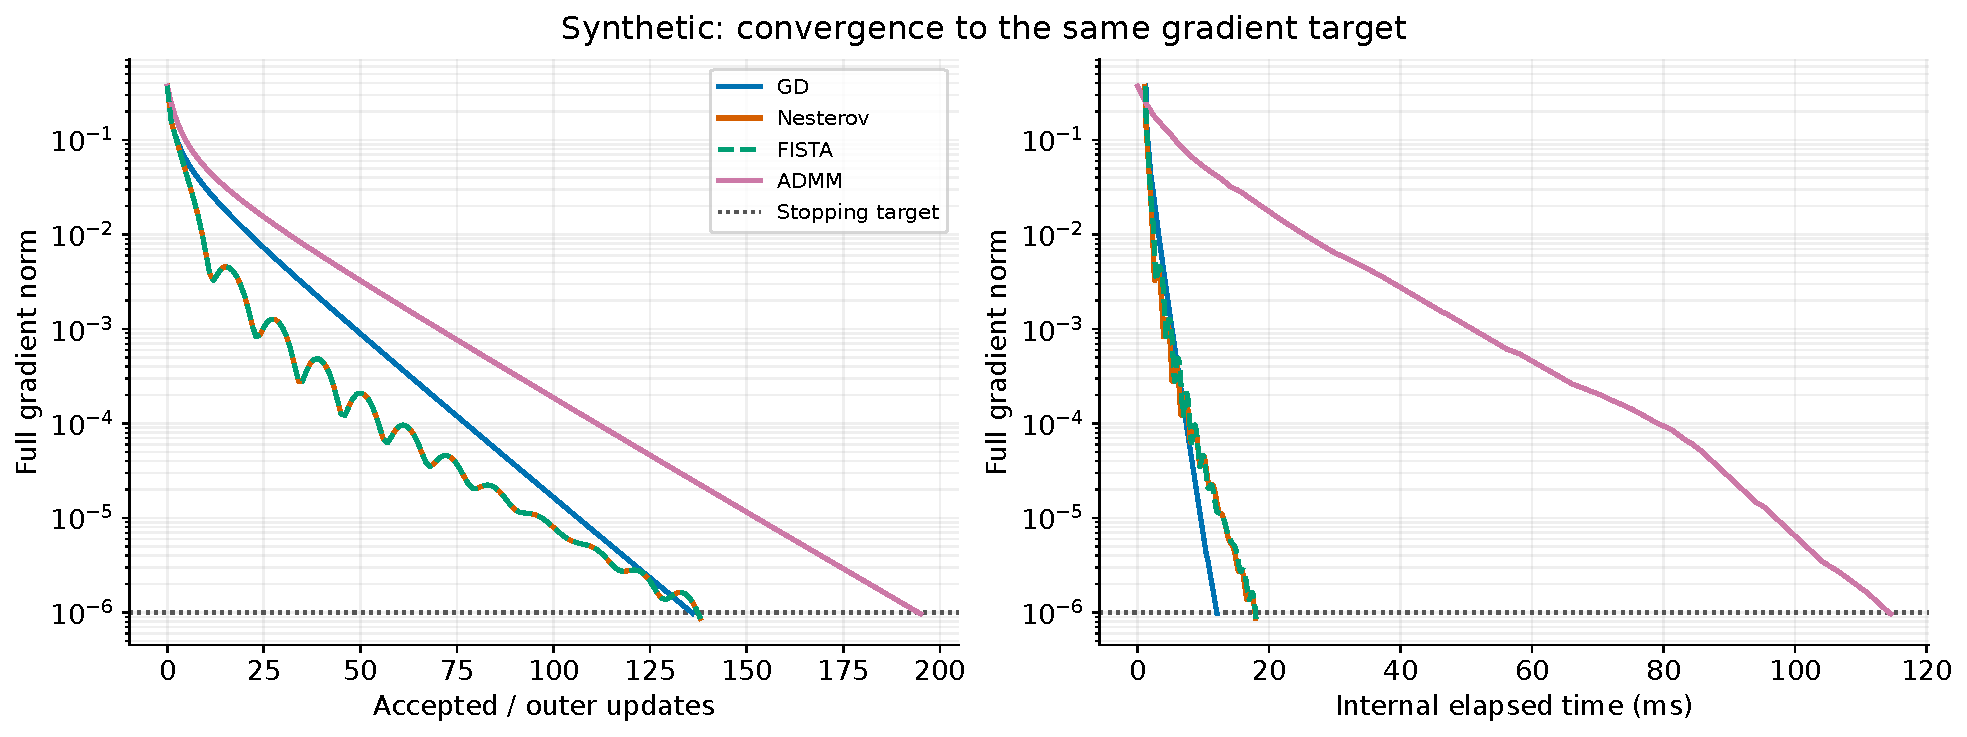
\includegraphics[width=\linewidth]{figures/synthetic_gradient.pdf}
\caption{Synthetic data: full gradient norm against updates (left) and time (right). The Nesterov and FISTA curves coincide, as predicted by \eqref{eq:equivalence}. The dotted line is the stopping target $10^{-6}$. Time curves come from the run whose wall time is closest to the median.}
\label{fig:synthetic}
\end{figure}

\paragraph{Breast cancer: momentum pays off.}
The picture changes on breast cancer (\cref{fig:breast}). GD needs 2{,}450 updates; Nesterov and FISTA need 1{,}172, fewer than half, and are the fastest in time even with two gradients per update. ADMM needs only 738 outer iterations, the fewest of all, but it is the slowest in time because those iterations contain 1{,}023 Newton steps. Ranking by iterations and ranking by time give different orders, so both views are needed.

\begin{figure}[t]
\centering
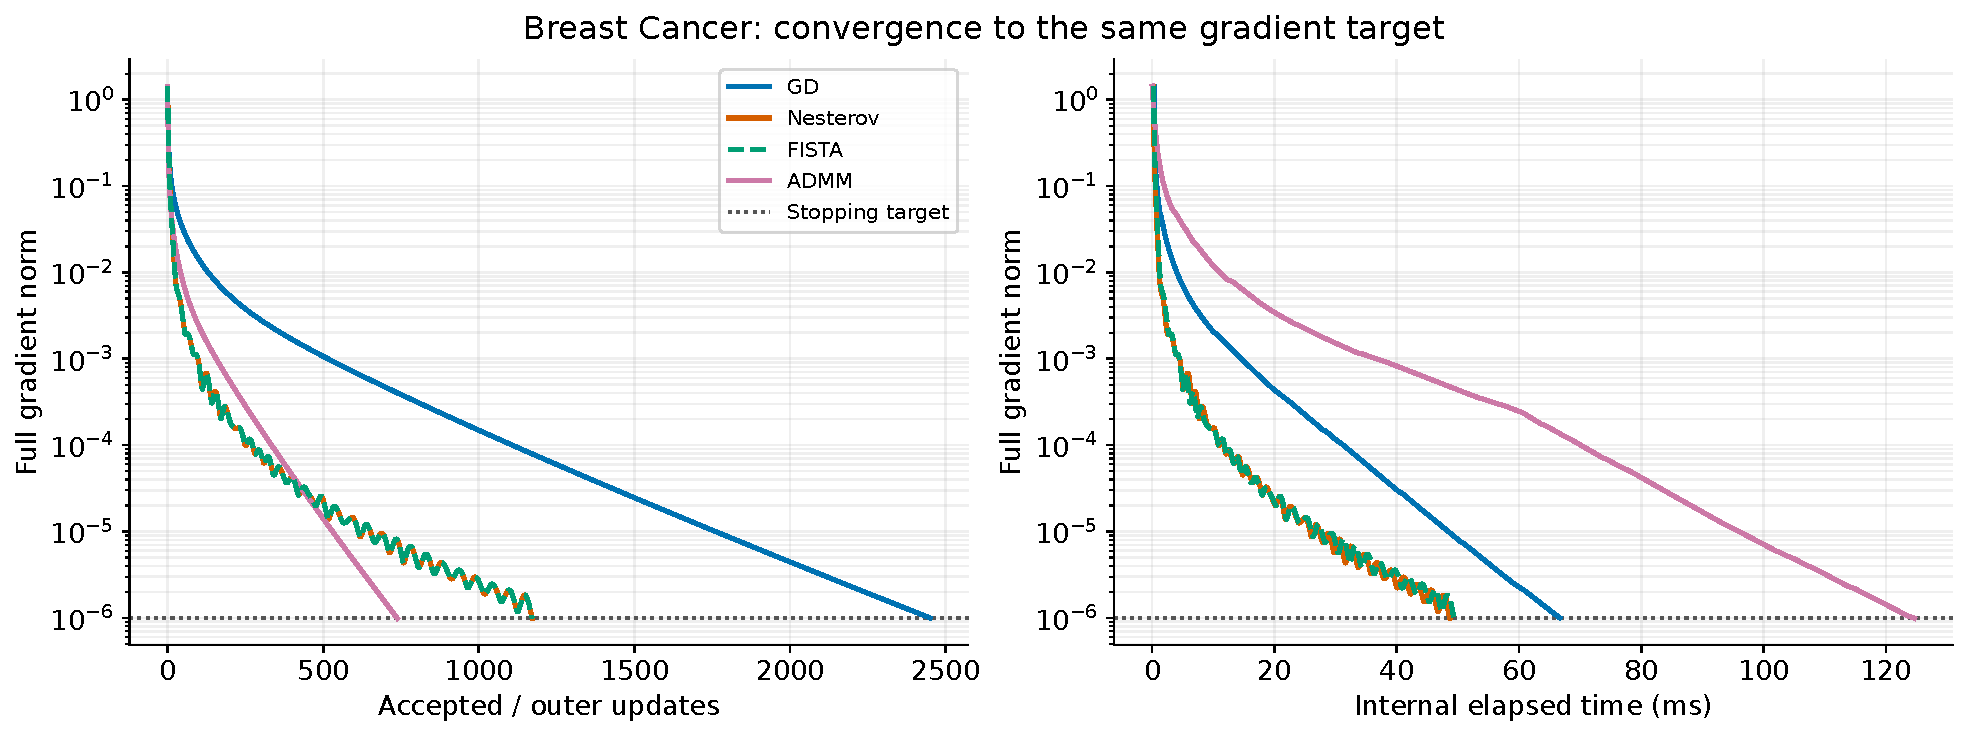
\includegraphics[width=\linewidth]{figures/breast_cancer_gradient.pdf}
\caption{Breast cancer: full gradient norm against updates (left) and time (right). ADMM uses the fewest outer updates but the most time; GD uses the most updates.}
\label{fig:breast}
\end{figure}

\paragraph{Timing spread.}
\Cref{fig:timing} shows the medians and IQRs. The spread is small relative to the gaps between methods, except for ADMM on breast cancer, whose upper quartile is noticeably higher. The difference between Nesterov and FISTA (under 1\,ms on breast cancer) is within implementation noise, since the two compute the same iterates; it says nothing about the algorithms.

\begin{figure}[t]
\centering
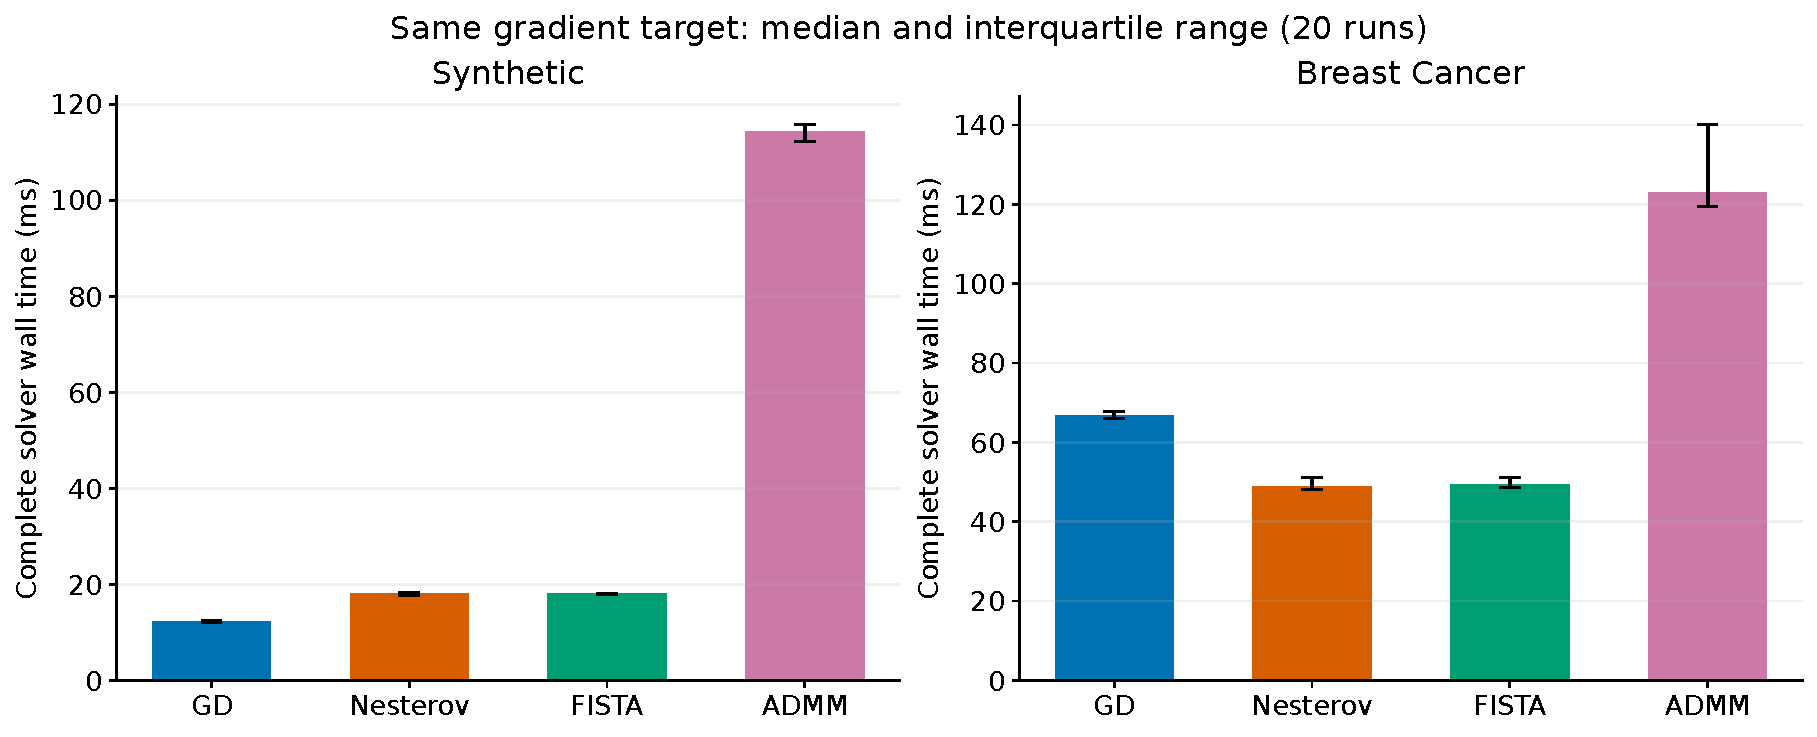
\includegraphics[width=0.92\linewidth]{figures/timing.pdf}
\caption{Wall time of the full solver call to the same gradient target: median and interquartile range over 20 runs.}
\label{fig:timing}
\end{figure}

\subsection{Why GD is slow on breast cancer}
\label{sec:why-gd}
The global bound $L/\mu$ is 75.0 on synthetic data and 334.6 on breast cancer (\cref{tab:conditioning}). One might conclude that breast cancer is simply worse conditioned. The Hessian at the solution says otherwise: its condition number is 47.8 on synthetic data but only 21.0 on breast cancer. The problem is not badly conditioned near $w^\star$; the step size is.

\begin{table}[t]
\caption{Global bounds and curvature at the solution $w^\star$ (seed 0, training design with bias). $\lambda_{\max}^\star$, $\lambda_{\min}^\star$ are the extreme eigenvalues of $\nabla^2F(w^\star)$.}
\label{tab:conditioning}
\centering
\small
\begin{tabular}{lrrrrrr}
\toprule
Dataset & $L$ & $L/\mu$ & $\lambda_{\max}^\star$ & $\lambda_{\min}^\star$ & $\lambda_{\max}^\star/\lambda_{\min}^\star$ & $L/\lambda_{\max}^\star$\\
\midrule
Synthetic     & 0.7497 & 74.97  & 0.4780 & 0.0100 & 47.80 & 1.57\\
Breast cancer & 3.3461 & 334.61 & 0.2104 & 0.0100 & 21.04 & 15.90\\
\bottomrule
\end{tabular}
\end{table}

$L$ assumes that every example has the largest possible logistic curvature, $p_i(1-p_i)=1/4$, which happens when $p_i=1/2$. Breast cancer is close to linearly separable: at the solution most training examples are classified with high confidence, $p_i$ is near $0$ or $1$, and the actual curvature is much smaller. As a result, $L$ is 15.9 times the largest Hessian eigenvalue at $w^\star$, against 1.57 on synthetic data. Near the solution, GD with step $1/L$ contracts the error along each eigendirection of $\nabla^2F(w^\star)$ by $1-\lambda_i^\star/L$. The slowest direction has $\lambda_{\min}^\star\approx\lambda=0.01$ on both datasets, so the effective condition number for fixed-step GD is $L/\lambda_{\min}^\star\approx335$ on breast cancer, while a step matched to the local curvature would face only $21$. On synthetic data the same comparison is $75$ against $48$. Accelerated methods depend on roughly the square root of the condition number when their momentum is well tuned, so a loose $L$ costs them less; this is consistent with Nesterov and FISTA needing about half as many updates as GD on breast cancer.

This explanation rests on measured curvature, not on a controlled ablation. A direct test would run GD with a locally adapted step, for example Barzilai--Borwein steps \citep{barzilai1988two}, and check whether the gap to the accelerated methods closes. We have not run that test.

\subsection{ADMM sensitivity to \texorpdfstring{$\rho$}{rho}}
\label{sec:rho}
\Cref{tab:rho} and \cref{fig:rho} vary $\rho$ with everything else fixed (5 timed repeats each). All settings converge, but the cost changes by more than two orders of magnitude. With $\rho=10$, ADMM needs 1{,}894 and 7{,}336 outer iterations and about one second. With $\rho=0.01$ it needs 18 and 19 iterations and a few milliseconds. Larger $\rho$ forces $w$ and $z$ together strongly in every step, so the iterates move slowly toward the optimum.

\begin{table}[t]
\caption{ADMM penalty sweep (seed 0, 5 repeats). All runs meet $\|\nabla F\|\le10^{-6}$. ``Newton'' is the total number of inner Newton steps.}
\label{tab:rho}
\centering
\small
\begin{tabular}{rrrrcrrr}
\toprule
& \multicolumn{3}{c}{Synthetic} & & \multicolumn{3}{c}{Breast cancer}\\
\cmidrule{2-4}\cmidrule{6-8}
$\rho$ & Outer & Newton & Time (ms) & & Outer & Newton & Time (ms)\\
\midrule
0.01 ($=\lambda$) & 18 & 5 & 4.08 & & 19 & 8 & 1.69\\
0.1  & 25 & 53 & 18.22 & & 78 & 137 & 14.80\\
1 (default) & 195 & 322 & 111.21 & & 738 & 1023 & 118.27\\
10   & 1894 & 2609 & 964.76 & & 7336 & 8497 & 1085.30\\
\bottomrule
\end{tabular}
\end{table}

\begin{figure}[t]
\centering
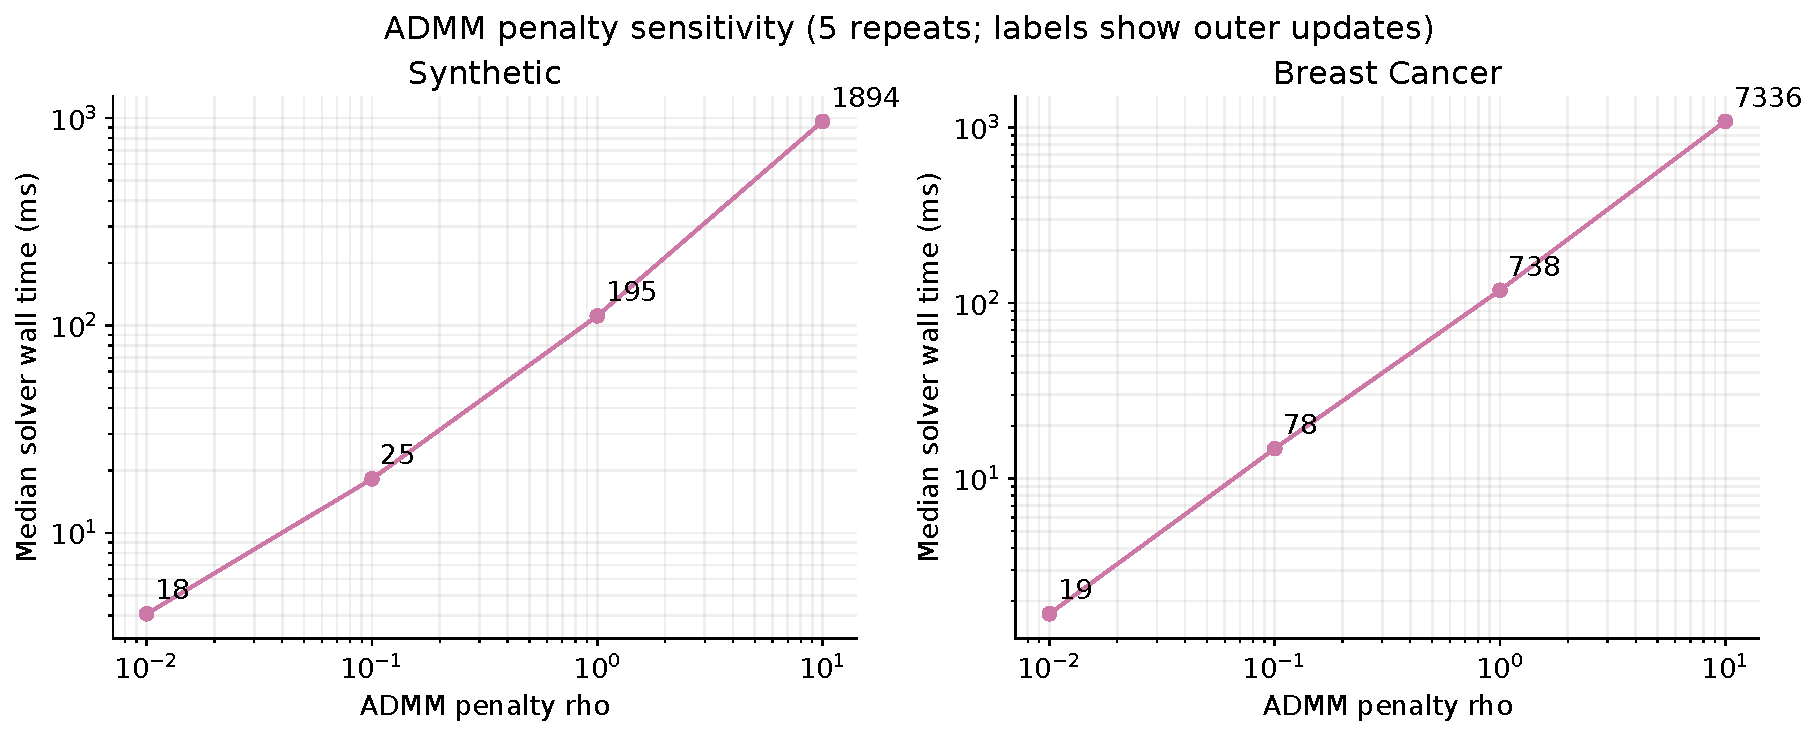
\includegraphics[width=0.85\linewidth]{figures/admm_rho.pdf}
\caption{ADMM median time against $\rho$ (log--log, 5 repeats). Labels give outer iterations.}
\label{fig:rho}
\end{figure}

\paragraph{The case $\rho=\lambda$ is special.}
The value $\rho=0.01$ is not a lucky setting; it equals $\lambda$. With $z_0=u_0=0$, the first subproblem \eqref{eq:admm-w} becomes $\min_w f(w)+\frac\lambda2\|w\|^2$, which is the original problem. The inner Newton solver therefore solves \eqref{eq:objective} during the first outer iteration (5 and 8 Newton steps; gradient norms $2.3\times10^{-12}$ and $9.3\times10^{-13}$). The $z$-update then gives $z_1=(w_1+u_0)/2$ and the dual update gives $u_1=z_1$, so $z-u$ stays zero and every later subproblem is unchanged. The remaining 17--18 outer iterations do no optimization; they only drive the primal and dual residuals below their thresholds.

\begin{figure}[t]
\centering
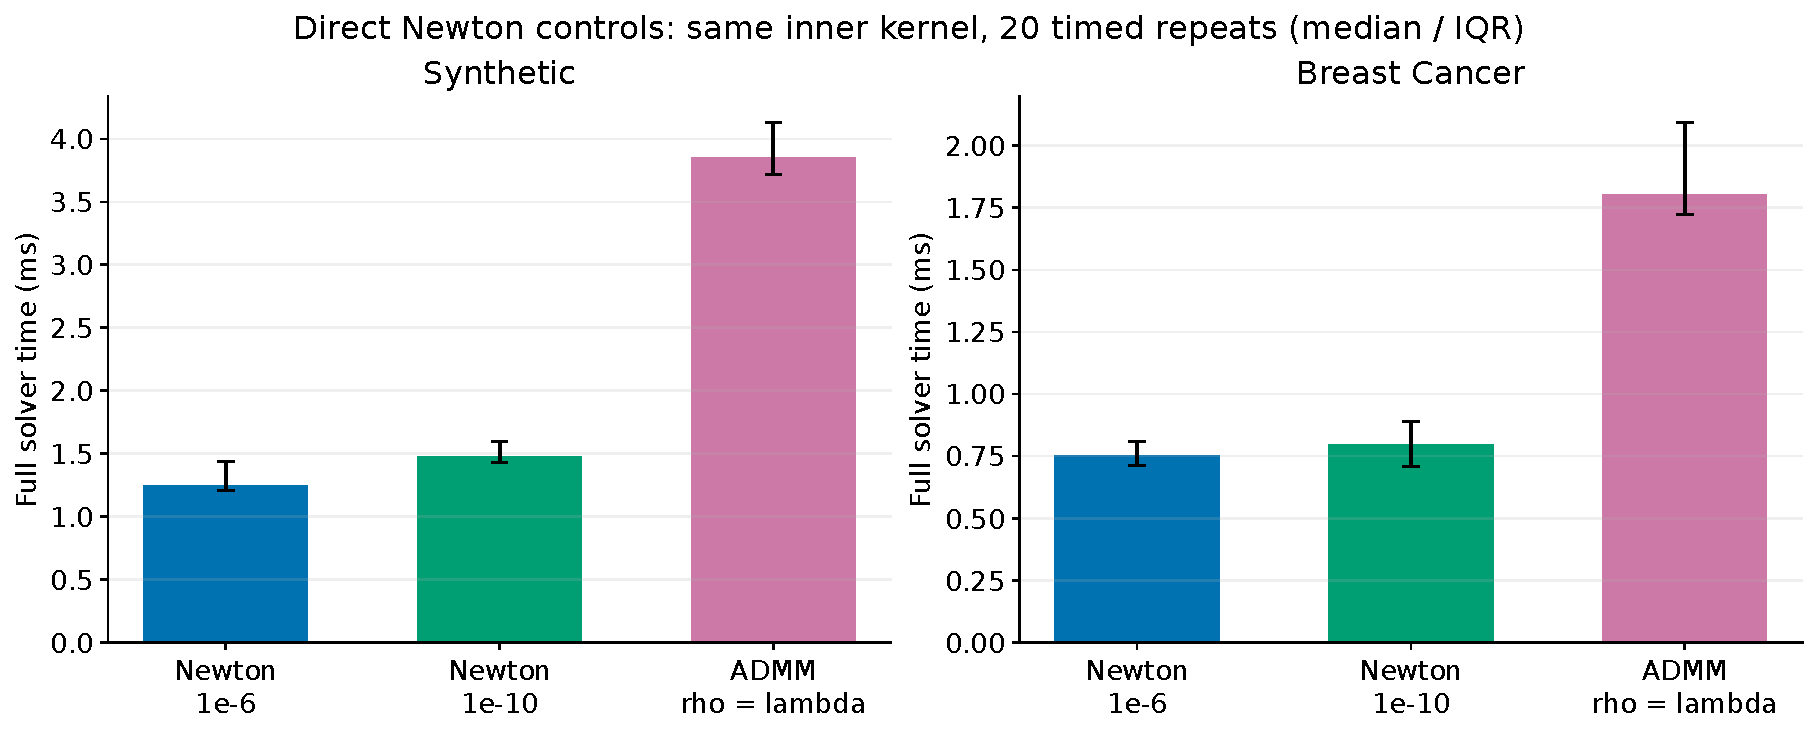
\includegraphics[width=0.85\linewidth]{figures/newton_controls.pdf}
\caption{Direct Newton on \eqref{eq:objective} at two tolerances, against ADMM with $\rho=\lambda$ (median and IQR, 20 repeats).}
\label{fig:newton}
\end{figure}

To check this, we ran Newton's method directly on \eqref{eq:objective}, using the same Newton routine as inside ADMM (\cref{fig:newton}). At tolerance $10^{-10}$ it takes 5 and 8 steps and about 1.5 and 0.8\,ms; ADMM with $\rho=\lambda$ takes 3.9 and 1.8\,ms. In this case ADMM is Newton's method plus the bookkeeping of its outer loop. Even at the common tolerance $10^{-6}$, Newton is at least ten times faster than the fastest first-order method on these problems, because $d\le51$ makes a dense Newton step cheap.

We chose the $\rho$ values by training convergence only, never by test accuracy, and the default comparison in \cref{tab:main} keeps $\rho=1$. We do not recommend $\rho=\lambda$ as a general rule: the effect depends on the zero start, the quadratic penalty and this particular split. In practice $\rho$ is adapted during the run, for example by residual balancing \citep{boyd2011admm}.

\subsection{Accuracy is not a convergence test}
\label{sec:budget}
With our original budget of 400 updates on breast cancer, no method met the tolerance: the final gradient norms were $1.7\times10^{-3}$ (GD), $4.2\times10^{-5}$ (Nesterov and FISTA) and $4.5\times10^{-5}$ (ADMM). Yet all four already had the final training and test accuracy, 99.06\% and 96.50\%. Accuracy depends only on the sign of each score, so it stops changing long before the weights converge. A run that looks finished by accuracy, or by a flat objective curve, may still be far from the optimum, and the gradient certificate \eqref{eq:certificate} is the reliable test. On synthetic data all methods met the tolerance within 400 updates.

\subsection{Robustness across data seeds}
We repeated the comparison for seeds 0--4 (\cref{tab:seeds}). On breast cancer the seed changes only the split; on synthetic data it changes both the generated data and the split. Every method converged in all 20 runs. Within each case all methods gave the same test accuracy. The ranking by updates on breast cancer is stable: ADMM fewest, then Nesterov/FISTA, then GD at about twice their count. On synthetic data GD's count varies more (136--198) than Nesterov's (138--168), so their order by updates is not fixed across seeds; we only have timing repeats for seed 0.

\begin{table}[t]
\caption{Seeds 0--4: converged runs, range of update counts, and range of test accuracy (identical across methods within each seed).}
\label{tab:seeds}
\centering
\small
\begin{tabular}{lcccc}
\toprule
& \multicolumn{2}{c}{Synthetic} & \multicolumn{2}{c}{Breast cancer}\\
\cmidrule(lr){2-3}\cmidrule(lr){4-5}
Method & Converged & Updates & Converged & Updates\\
\midrule
GD       & 5/5 & 136--198 & 5/5 & 2339--2450\\
Nesterov & 5/5 & 138--168 & 5/5 & 1127--1192\\
FISTA    & 5/5 & 138--168 & 5/5 & 1127--1192\\
ADMM     & 5/5 & 195--233 & 5/5 & 700--738\\
\midrule
Test accuracy & \multicolumn{2}{c}{73.80--83.60\%} & \multicolumn{2}{c}{96.50--97.90\%}\\
\bottomrule
\end{tabular}
\end{table}

\subsection{Correctness checks}
Besides the Nesterov--FISTA overlap, we verified every endpoint against an independent damped Newton solve: all 54 saved endpoints agree within the objective-gap bound \eqref{eq:certificate}. The 400-update results were reproduced exactly in the later timing batch.

%======================================================================
\section{Discussion and conclusions}
\label{sec:conclusion}

\paragraph{Main findings.}
\begin{enumerate}
\item \emph{There is no single winner.} GD is the fastest on synthetic data; Nesterov and FISTA are the fastest on breast cancer. Which one wins depends on how loose the global step bound is near the solution, which we measured directly (\cref{tab:conditioning}).
\item \emph{FISTA and Nesterov coincide for an L2 penalty.} The identity \eqref{eq:equivalence} predicts this, and the measured trajectories confirm it. FISTA becomes a different method only for nonsmooth penalties such as L1.
\item \emph{Iteration counts can mislead.} ADMM needs the fewest outer iterations on breast cancer but the most time, because each iteration hides dense Newton work. Nesterov and FISTA need twice the gradient evaluations per update of GD.
\item \emph{ADMM depends heavily on $\rho$.} Over $\rho\in[0.01,10]$ its time changes by more than two orders of magnitude, and at $\rho=\lambda$ it reduces to Newton's method.
\item \emph{Accuracy converges long before the optimizer.} A gradient-based certificate is needed to decide that training is finished.
\end{enumerate}

\paragraph{Strengths and weaknesses.}
\Cref{tab:procon} summarizes what we would tell a practitioner. For problems of this size, Newton's method is the best choice. With $d$ in the hundreds of thousands, as in text classification, a dense Newton step becomes impossible and first-order or quasi-Newton methods such as L-BFGS \citep{liu1989limited} take over.

\begin{table}[t]
\caption{Strengths, weaknesses and use cases, based on the analysis and our measurements.}
\label{tab:procon}
\centering
\small
\begin{tabular}{p{1.3cm}p{3.5cm}p{3.8cm}p{3.4cm}}
\toprule
Method & Strengths & Weaknesses & Use when\\
\midrule
GD & Simple, monotone, one gradient per update; easy to verify & Step $1/L$ can be very conservative; rate depends on $L/\mu$ & Baseline; well-conditioned or tight-$L$ problems\\
Nesterov & $O(1/k^2)$ rate; large gains when $L$ is loose & Oscillates without restart or $\mu$-tuned momentum; two gradients per update in our code & Smooth objectives where GD is slow\\
FISTA & Handles nonsmooth penalties through a cheap prox & Identical to Nesterov for L2; same oscillation & L1, elastic net, constraints with simple projections\\
ADMM & Splits loss and penalty; suits distributed and constrained problems & Sensitive to $\rho$; expensive subproblems & Data spread over machines; structured constraints\\
\bottomrule
\end{tabular}
\end{table}

\paragraph{Limitations.}
We used two small, dense datasets on one machine, so the absolute times and the ranking do not transfer to large or sparse data. Only one value of $\lambda$ was tested; a larger $\lambda$ lowers $L/\mu$ and would speed up every method. Our Nesterov and FISTA use the general-convex momentum without restart, which is not the best accelerated variant for a strongly convex problem. ADMM uses a strict inner tolerance of $10^{-10}$; an inexact version with a looser, gradually tightened tolerance would likely be faster. The explanation of GD's slowness is based on measured curvature rather than an ablation.

\paragraph{Future work.}
(i) Add strongly convex momentum and adaptive restart \citep{odonoghue2015adaptive} to test whether the oscillations in \cref{fig:synthetic} disappear. (ii) Run GD with Barzilai--Borwein or backtracking-from-above steps to test the step-size explanation in \cref{sec:why-gd}. (iii) Sweep $\lambda$ to vary conditioning. (iv) Replace the L2 penalty by L1, where FISTA and Nesterov separate. (v) Test inexact ADMM and residual balancing for $\rho$, and a genuinely distributed consensus split.

\paragraph{Reproducibility.}
All code, raw timings, histories and environment records are in the repository. The experiments are reproduced by:
\begin{itemize}
\item \texttt{experiments/run\_compare.py}: the original 400-update comparison;
\item \texttt{experiments/supplement.py}: same-precision runs, the $\rho$ sweep and the seed study;
\item \texttt{experiments/newton\_comparison.py}: the timing batch, Newton controls and conditioning;
\item \texttt{experiments/verify\_newton.py}, \texttt{verify\_supplement.py}: independent endpoint checks.
\end{itemize}
Figures are generated from the saved \texttt{raw.json} files.

\paragraph{Contributions of members.}
WANG Zeqing implemented GD and wrote the background survey. LIU Xuyang implemented Nesterov's method and wrote the problem formulation and conclusions. WU Aoqi implemented FISTA, wrote the methodology, and built the experiment and figure scripts. ZHAO Jixin implemented ADMM and wrote the experimental analysis. All members contributed to the presentation.

\bibliographystyle{plainnat}
\bibliography{refs}

\end{document}
